\documentclass[a4paper,12pt]{article}
\usepackage[utf8]{inputenc}
\usepackage[english]{babel}
\usepackage[T1]{fontenc} % for correct << and >>
\usepackage{amssymb, amsmath, multicol, amsthm, mathtools}
\usepackage{csquotes}
\usepackage{mathrsfs}
\usepackage{graphicx}
\usepackage{multirow}
\usepackage{caption}
\usepackage{subcaption}
\usepackage{indentfirst}
\usepackage{esvect}
\usepackage{float} 
\usepackage[version=4]{mhchem}
\mathtoolsset{showonlyrefs=true}
\usepackage{hyperref}
\usepackage[rgb,table,xcdraw]{xcolor}
\hypersetup{				
	unicode=true,        
	colorlinks=true,       	
	linkcolor=black,        
	citecolor=black,        
	filecolor=magenta,      
	urlcolor=black         
}

\usepackage[left=2cm,right=2cm,
    top=2cm,bottom=2cm]{geometry}
\usepackage{fancyhdr}


\graphicspath{{images}}

\newcommand{\angstrom}{\text{\normalfont\AA}}
\newcommand{\iu}{\mathrm{i}\mkern1mu}
\newcommand*{\hatH}{\hat{\mathcal{H}}}


\begin{document}

    \section{Definition of the Hamiltonian}

        There is a number of details in the definition of the Heisenberg Hamiltonians, which may cause an incompatibility of the direct results. 
        In this paper the main definition is as follows:

        \begin{equation}
            \hat{H} = -J \sum_{ij} \hat{\mathbf{S}}_i^T \hat{\mathbf{S}}_j
            \label{eq:hh-main}
        \end{equation}
        where $J$ is an isotropic exchange parameter. The double counting is present in the Hamiltonian, i.e. both terms $i\rightarrow j$ and $j \rightarrow i$ are present in the sum. 
        $\hat{\mathbf{S}}_i$ is a $3\times1$ column vector of the spin operators $(\hat{\mathbf{S}}_i^x, \hat{\mathbf{S}}_i^y, \hat{\mathbf{S}}_i^z)$. 
        Index $i$ run over all $N$ sites in the system and index $j$ runs over neighbors for the site $i$. 

        Bold mathematical symbols in this work represent vectors or matrices and usual symbols - scalars. For instance, $J$ is a scalar exchange parameter, while $\mathbf{J}$ is a matrix of exchange, 
        for the isotropic case it is defined as

        \begin{equation}
            \mathbf{J} =
            \begin{pmatrix}
                J & 0 & 0 \\
                0 & J & 0 \\
                0 & 0 & J
            \end{pmatrix}
        \end{equation}

        Several comparisons of the exchange Hamiltonians and consecutive spin wave Hamiltonians will be done in this paper and for each one the details of the convergence will be discussed. 
        When possible the results will be present in both ways: the original source and in the definition of this paper.

    \section{Ferromagnetic cubic system}

        In this section I will define the parameters and they values for the case study system - 
        cubic lattice of ferromagnetic spins oriented along the direction of $z$ axis.

        Lattice (see~Fig.~\ref{fig:lattice}) in cartesian coordinate system is defined by the lattice parameters and angles:
        \begin{equation}
            \begin{matrix}
                \mathbf{a} = (l, 0, 0) & \mathbf{b} = (0, l, 0) & \mathbf{c} = (0, 0, l) \\
                \alpha = 90^{\circ} & \beta = 90^{\circ} & \gamma = 90^{\circ} \\
            \end{matrix}
        \end{equation}
        In each unit cell there is one spin $S$ at the position $(0, 0, 0)$ (in relative coordinates).

        Spin in the $(0, 0, 0)$ unit cell will have 6 neighbors as shown in Fig.~\ref{fig:lattice-neighbors}.

        \begin{figure}[H]
            \centering
            \begin{subfigure}[b]{0.49\textwidth}
                \centering
                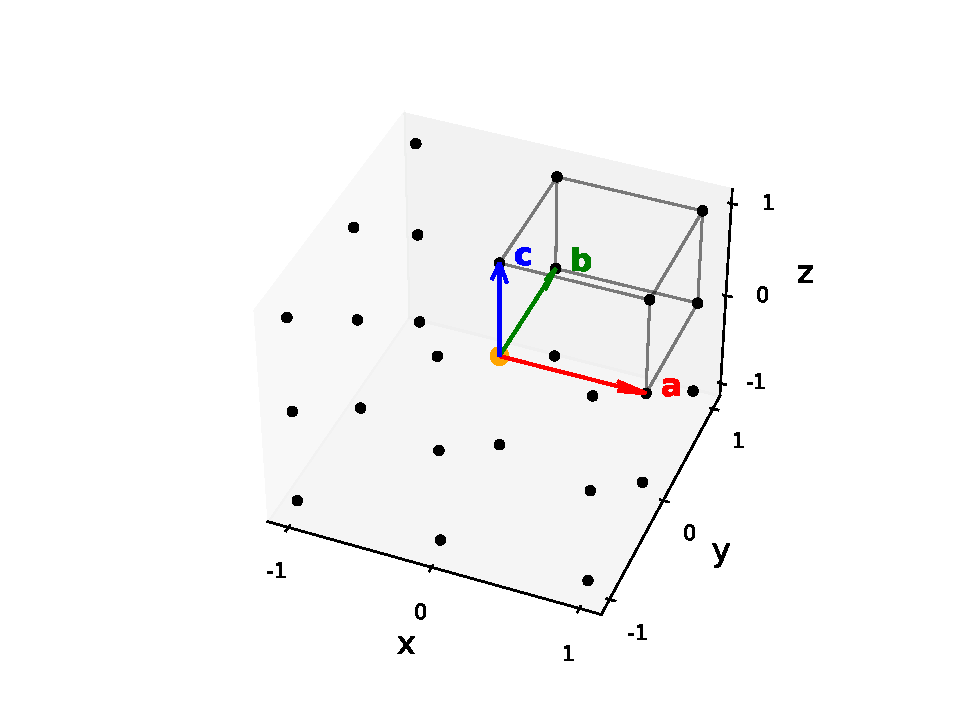
\includegraphics[height=6cm]{lattice.pdf}
                \caption{}
            \label{fig:lattice}
            \end{subfigure}
            \hfill
            \begin{subfigure}[b]{0.49\textwidth}
                \centering
                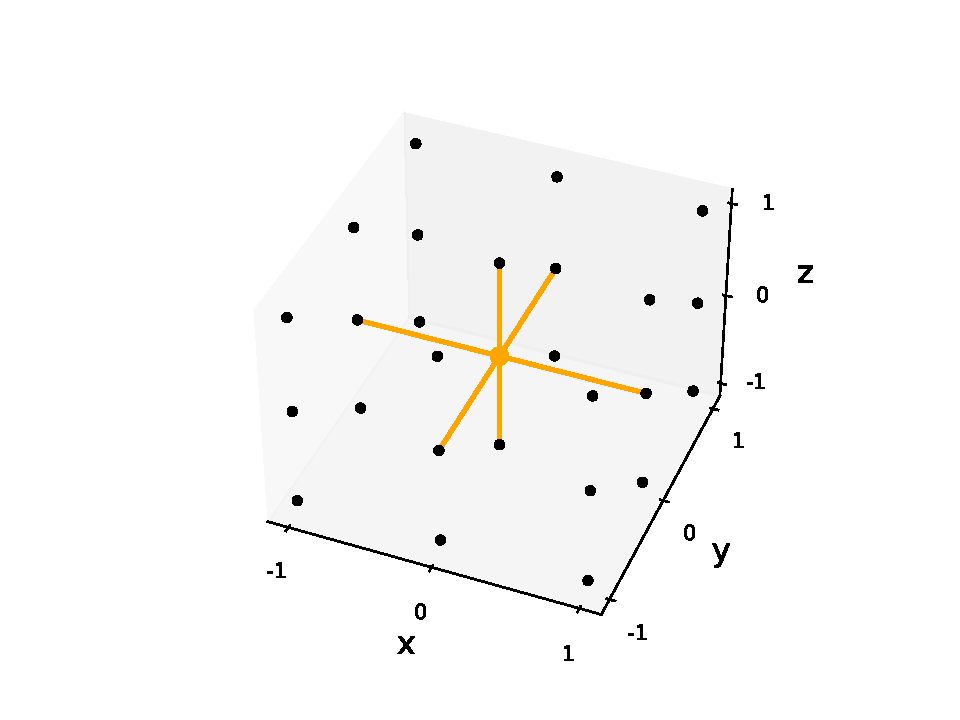
\includegraphics[height=6cm]{lattice-neighbors.pdf}
            \caption{}
            \label{fig:lattice-neighbors}
            \end{subfigure}
            \hfill
            \caption{(a) Lattice and (b) 6 neighbors for the spin in $(0, 0, 0)$ unit cell.}
            \label{fig:lattice-both}
        \end{figure}


        The reciprocal lattice will have the form of:
        \begin{equation}
            \begin{matrix}
                \mathbf{b_1} = (\dfrac{2\pi}{l}, 0, 0) & \mathbf{b_2} = (0,\dfrac{2\pi}{l}, 0) & \mathbf{b_3} = (0, 0, \dfrac{2\pi}{l}) \\
                k_{\alpha} = 90^{\circ} & k_{\beta} = 90^{\circ} & k_{\gamma} = 90^{\circ} \\
            \end{matrix}
        \end{equation}

        Magnon dispersion plots will use the following path: Y-$\Gamma$-X-M-$\Gamma$-R-X$\vert$M-R (see~Fig.~\ref{fig:path}).

        \begin{figure}[H]
            \centering
            \begin{subfigure}[b]{0.8\textwidth}
                \centering
                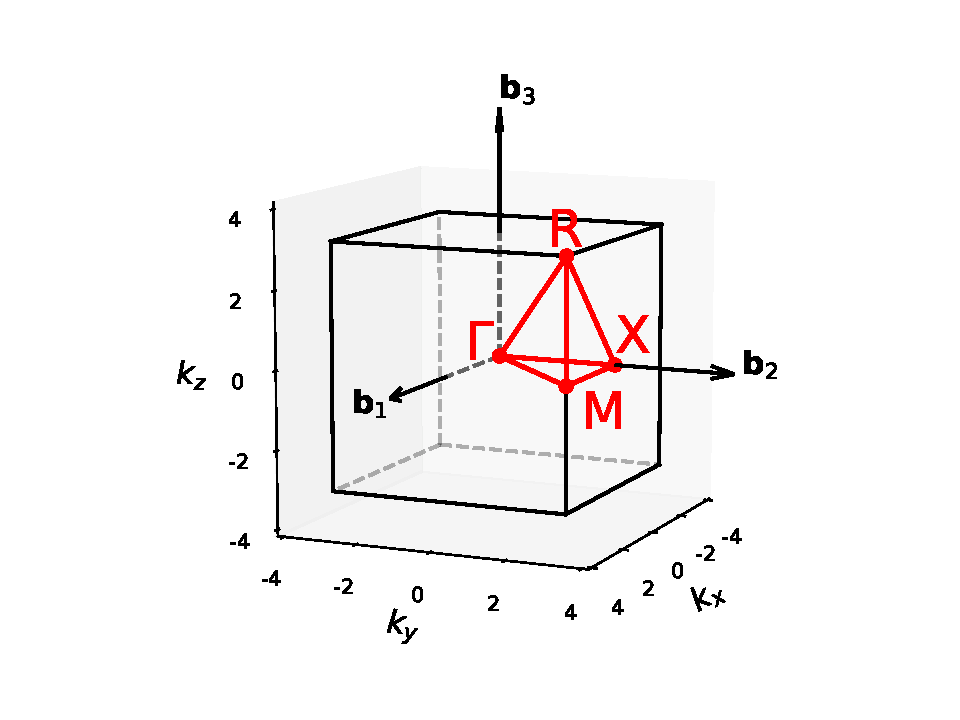
\includegraphics[height=10cm]{path.pdf}
            \end{subfigure}
            \hfill
            \caption{Path in reciprocal space for the magnon dispersion plot: Y-$\Gamma$-X-M-$\Gamma$-R-X$\vert$M-R.}
            \label{fig:path}
        \end{figure}


        For the final results and for the Figs.~\ref{fig:lattice-both}~and~\ref{fig:path} the following numerical values are used:
        \begin{equation}
            \begin{matrix}
                J = 1 \text{ meV}, & S = 1, & l = 1, & n = 6
            \end{matrix}
        \end{equation}

    \section{Main magnon dispersion}

        In Appendix I magnon dispersion is derived from the Hamiltonian~in~\eqref{eq:hh-main}.
        The final result is present in equation~\ref{eq:main-dispersion}. 

        \begin{equation}
            \boxed{
            \hbar\omega(\mathbf{k}) = 2JSn\left(1 - 
            \dfrac{1}{3}\left(\cos(k_x l) + \cos(k_y l) + \cos(k_z l)\right)\right)}
            \label{eq:main-dispersion}
        \end{equation}

        In Fig.~\ref{fig:main-dispersion} is plotted for the path Y-$\Gamma$-X-M-$\Gamma$-R-X$\vert$M-R. 
        The picture is produced with the script <<codes/dispersion.py>> using 
        <<main\_dispersion>> function.


        \begin{figure}[H]
            \centering
            \begin{subfigure}[b]{0.8\textwidth}
                \centering
                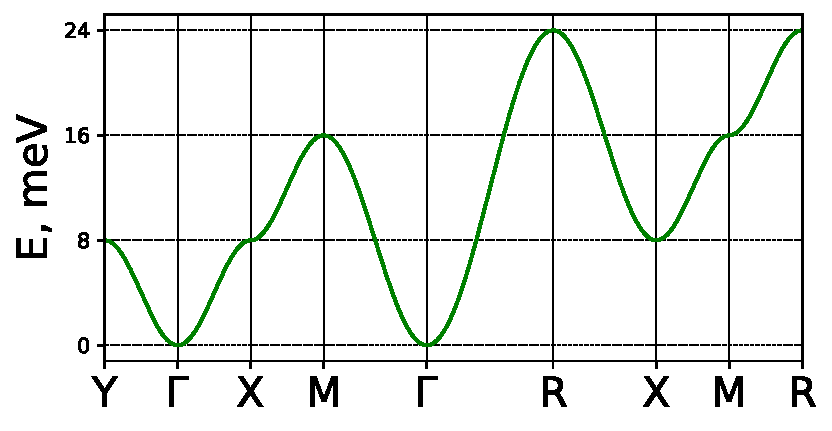
\includegraphics[height=7cm]{main_dispersion.pdf}
            \end{subfigure}
            \hfill
            \caption{Magnon dispersion plotted with equation~\eqref{eq:main-dispersion}.}
            \label{fig:main-dispersion}
        \end{figure}

        \section{Literature check}
        In this section I will compare the result in equation~\eqref{eq:main-dispersion} with the textbook results. 
        For each source Hamiltonian definitions are compared with the equation~\eqref{eq:hh-main} and make conversion if necessary. 
        Detail consideration of each source is provided in Appendix~II. In Table~\ref{tab:literature-review} the summary of textbooks review is provided.

        \begin{table}[H]
            \centering
            \caption{Comparasion of magnon dispersion formulas with textbooks (converted to the notation of this paper).}
            \label{tab:literature-review}
            \def\arraystretch{2.5}
            \begin{tabular}{|c|c|}
            \hline
            Source                             & Formula                                                                                                        \\ \hline
            This paper                         & $\hbar\omega(\mathbf{k}) = 2JSn\left(1 - \dfrac{1}{3}\left(\cos(k_xl) + \cos(k_yl) + \cos(k_zl)\right)\right)$ \\ \hline
            \cite{rezende2020fundamentals}     & $\hbar\omega(\mathbf{k}) = 2nJS\left(1 - \dfrac{1}{3}\left(\cos(k_xl) + \cos(k_yl) + \cos(k_zl)\right)\right)$ \\ \hline
            \cite{blundell2003magnetism}       & $\hbar\omega(\mathbf{k}) = 2nJS\left(1 - \dfrac{1}{3}\left(\cos(k_xl) + \cos(k_yl) + \cos(k_zl)\right)\right)$ \\ \hline
            \cite{gurevich1996magnetization}   & $\hbar\omega(\mathbf{k}) = 2SJn\left(1 - \dfrac{1}{3}\left(\cos(k_xl) + \cos(k_yl) + \cos(k_zl)\right)\right)$ \\ \hline
            \cite{simon2013oxford}             & $\hbar\omega(\mathbf{k}) = 2JSn\left(1 - \dfrac{1}{3}\left(\cos(k_xl) + \cos(k_yl) + \cos(k_zl)\right)\right)$ \\ \hline
            \cite{coey2010magnetism}           & $\hbar\omega(\mathbf{k}) = 2JSn\left(1 - \dfrac{1}{3}\left(\cos(k_xl) + \cos(k_yl) + \cos(k_zl)\right)\right)$ \\ \hline
            \cite{jensen1991rare}              & $\hbar\omega(\mathbf{k}) = Sn2J\left(1 - \dfrac{1}{3}\left(\cos(k_xl) + \cos(k_yl) + \cos(k_zl)\right)\right)$ \\ \hline
            \end{tabular}
            \end{table}

    \section{Appendix I}

In this section The magnon dispersion law is derived from the Hamiltonian in eq.~\eqref{eq:hh-main}.
First of all, the Hamiltonian is rewritten with the raising and lowering spin operators:

\begin{equation}
    \hat{S}_i^{\pm} = \hat{S}_i^x \pm \iu \hat{S}_i^y
\end{equation}

\begin{equation}
    \begin{matrix}
        \hat{\mathbf{S}}_i^T \hat{\mathbf{S}}_j = 
        \hat{S}_i^x \hat{S}_j^x + \hat{S}_i^y \hat{S}_j^y + \hat{S}_i^z \hat{S}_j^z; &
        \hat{S}_i^x \hat{S}_j^x + \hat{S}_i^y \hat{S}_j^y = 
        \dfrac{1}{2}\left(\hat{S}_i^+\hat{S}_j^- + \hat{S}_i^-\hat{S}_j^+\right)
    \end{matrix}
\end{equation}

\begin{equation}
    \hat{H} = -J \sum_{ij} \left(\dfrac{1}{2}\left(
        \hat{S}_i^+\hat{S}_j^- + \hat{S}_i^-\hat{S}_j^+\right) + \hat{S}_i^z \hat{S}_j^z\right)
\end{equation}

Since the commutator is 
\begin{equation}
    \left[\hat{S}_i^+\hat{S}_j^-\right] = 2\hat{S}_i^z\delta_{ij}
\end{equation}
and $i\ne j$ in the sum the Hamiltonian becomes:
\begin{equation}
    \hat{H} =-J \sum_{ij} \left(\dfrac{1}{2}\left(
            \hat{S}_j^-\hat{S}_i^+ + \hat{S}_i^-\hat{S}_j^+\right) + \hat{S}_i^z \hat{S}_j^z\right)
\end{equation}

The spin-wave Hamiltonian is obtained with the linearised Holstein–Primakoff formalism.

\begin{equation}
    \begin{matrix}
        \hat{S}_i^+ = \sqrt{2S}\hat{a}_i \\
        \hat{S}_i^- = \sqrt{2S}\hat{a}_i^{\dag} \\
        \hat{S}_i^z = S - \hat{a}_i^{\dag}\hat{a}_i
    \end{matrix}
\end{equation}

\begin{equation}
    \hat{H} = -J \sum_{ij} \left(\dfrac{1}{2}\left(
        2S\hat{a}_j^{\dag}\hat{a}_i + 2S\hat{a}_i^{\dag}\hat{a}_j\right) + 
        \left(S - \hat{a}_i^{\dag}\hat{a}_i\right)\left(S - \hat{a}_j^{\dag}\hat{a}_j\right)\right)
\end{equation}

\begin{equation}
    \hat{H} = E_0 + \hat{H}^{(2)} + \dots 
\end{equation}
\begin{equation}
    E_0 = -JS^2Nn \label{eq:zero-energy}
\end{equation}
\begin{equation}
    \hat{H}^{(2)} = -JS \sum_{ij} \left(\hat{a}_j^{\dag}\hat{a}_i + \hat{a}_i^{\dag}\hat{a}_j - 
    \hat{a}_i^{\dag}\hat{a}_i - \hat{a}_j^{\dag}\hat{a}_j\right)
    \label{eq:quadratic-ham}
\end{equation}
where $N$ is the number of spins in the system, $n$ - number of neighbors for each spin ($6$ in the case of cubic system).
From this point the quadratic part of the Hamiltonian $\hat{H}^{(2)}$ is considered.

The Fourier transform is introduced to move from the local operators $\hat{a}_i^{\dag}$ and $\hat{a}_i$
to the collective creation and annihilation operators $\hat{a}_k^{\dag}$ and $\hat{a}_k$:
\begin{equation}
    \hat{a}_i = \dfrac{1}{\sqrt{N}}\sum_k e^{\iu\mathbf{k}\mathbf{r}_i} \hat{a}_k 
\end{equation}
\begin{equation}
    \hat{a}_i^{\dag} = \dfrac{1}{\sqrt{N}}\sum_k e^{-\iu\mathbf{k}\mathbf{r}_i} \hat{a}_k^{\dag} 
\end{equation}
\begin{equation}
    \dfrac{1}{N}\sum_i e^{\iu(\mathbf{k} - \mathbf{k}^{\prime})\mathbf{r}_i} = \delta_{kk^{\prime}} 
\end{equation}

\begin{equation}
\begin{aligned}
    \hat{H}^{(2)}  = -JS \sum_i\sum_j \dfrac{1}{N}\left[
        \left(\sum_k e^{-\iu\mathbf{k}\mathbf{r}_j} \hat{a}_k^{\dag}\right)
        \left(\sum_{k^{\prime}} e^{\iu\mathbf{k^{\prime}}\mathbf{r}_i} \hat{a}_{k^{\prime}}\right)\right. \\
        +
        \left(\sum_k e^{-\iu\mathbf{k}\mathbf{r}_i} \hat{a}_k^{\dag}\right)
        \left(\sum_{k^{\prime}} e^{\iu\mathbf{k^{\prime}}\mathbf{r}_j} \hat{a}_{k^{\prime}}\right)  \\
        -
        \left(\sum_k e^{-\iu\mathbf{k}\mathbf{r}_i} \hat{a}_k^{\dag}\right)
        \left(\sum_{k^{\prime}} e^{\iu\mathbf{k^{\prime}}\mathbf{r}_i} \hat{a}_{k^{\prime}}\right)  \\
        -
        \left.\left(\sum_k e^{-\iu\mathbf{k}\mathbf{r}_j} \hat{a}_k^{\dag}\right)
        \left(\sum_{k^{\prime}} e^{\iu\mathbf{k^{\prime}}\mathbf{r}_j} \hat{a}_{k^{\prime}}\right) \right]
\end{aligned}
\end{equation}

Since for each $i$ there is the same pattern of neighbors sum over $j$ does not depend on $i$ and it can be moved freely.
Lets define $\boldsymbol{\delta}_j = \mathbf{r}_j - \mathbf{r}_i$ and rewrite the equation:

\begin{equation}
\begin{aligned}
    \hat{H}^{(2)}  = -JS \sum_k\sum_{k^{\prime}}\sum_j \left[
        e^{-\iu\boldsymbol{\delta}_j\mathbf{k}}
        \left(\dfrac{1}{N}\sum_ie^{\iu(\mathbf{k^{\prime}}-\mathbf{k})\mathbf{r}_i}\right) 
        \hat{a}_k^{\dag}\hat{a}_{k^{\prime}}\right. \\
        +
        e^{\iu\boldsymbol{\delta}_j\mathbf{k}}
        \left(\dfrac{1}{N}\sum_ie^{\iu(\mathbf{k^{\prime}}-\mathbf{k})\mathbf{r}_i}\right)
         \hat{a}_k^{\dag}\hat{a}_{k^{\prime}}  \\
        -
        \left(\dfrac{1}{N}\sum_ie^{\iu(\mathbf{k^{\prime}}-\mathbf{k})\mathbf{r}_i}\right)
        \hat{a}_k^{\dag}\hat{a}_{k^{\prime}}  \\
        -
        \left.e^{\iu(\mathbf{k^{\prime}}-\mathbf{k})\boldsymbol{\delta}_j}
        \left(\dfrac{1}{N}\sum_ie^{\iu(\mathbf{k^{\prime}}-\mathbf{k})\mathbf{r}_i}\right)
        \hat{a}_k^{\dag}\hat{a}_{k^{\prime}} \right]
\end{aligned}
\end{equation}
every equation in round parenthesis is equal to $\delta_{kk^{\prime}}$ and the Hamiltonian becomes

\begin{multline}
    \hat{H}^{(2)} = -JS\sum_k\sum_j\left[e^{-\iu\boldsymbol{\delta}_j\mathbf{k}}
    \hat{a}_k^{\dag}\hat{a}_k
    +
    e^{\iu\boldsymbol{\delta}_j\mathbf{k}}
     \hat{a}_k^{\dag}\hat{a}_k 
    -
    \hat{a}_k^{\dag}\hat{a}_k 
    -
    e^{\iu(\mathbf{k}-\mathbf{k})\boldsymbol{\delta}_j}
    \hat{a}_k^{\dag}\hat{a}_k\right] \\
     = 2JS\sum_k\sum_j(1 - \cos(\boldsymbol{\delta}_j\mathbf{k}))\hat{a}_k^{\dag}\hat{a}_k
\end{multline}
$j$ runs from $1$ to $n$, therefore:
\begin{equation}
    \hat{H}^{(2)} = 2JSn\sum_k\left(1 - \dfrac{1}{n}\sum_j
    \cos(\boldsymbol{\delta}_j\mathbf{k})\right)\hat{a}_k^{\dag}\hat{a}_k = 
    \sum_k \hbar\omega(\mathbf{k})\hat{a}_k^{\dag}\hat{a}_k
\end{equation}

For the cubic system ($l$ - length of the lattice vector):
\begin{align}
    \dfrac{1}{n}\sum_j
    e^{\iu\boldsymbol{\delta}_j\mathbf{k}}  = \dfrac{1}{6}\left(\cos(k_xl) + \cos(-k_xl) + \cos(k_yl) + \cos(-k_yl) + \cos(k_zl) + \cos(-k_zl)\right) \\
    = \dfrac{1}{3}\left(\cos(k_x l) + \cos(k_y l) + \cos(k_z l)\right)
\end{align}
and the final formula for the magnon dispersion is
\begin{equation}
    \hbar\omega(\mathbf{k}) = 2JSn\left(1 - 
    \dfrac{1}{3}\left(\cos(k_x l) + \cos(k_y l) + \cos(k_z l)\right)\right)
\end{equation}

    \section{Appendix II}

\subsection{<<Fundamentals of Magnonics>>\cite{rezende2020fundamentals}}

    In <<Fundamentals of Magnonics>> the derivation of magnon dispersion is done in chapter~$3$~<<Quantum Theory of Spin Waves: Magnons>>.

    The Hamiltonian is defined on page~$72$, equation~\eqref{eq:fom-3.6} as follows:

    \begin{quote}
        \begin{equation}
            H = -g\mu_B\sum_iH_zS_i^z - J\sum_{i, \delta}\vec{S}_i \cdot \vec{S}_{i+\delta}, \label{eq:fom-3.6} \tag{3.6}
        \end{equation}
        where$\vec{S}_i$ is spin angular momentum operator as site $i$, <...> and $\vec{\delta}$ is the vector connecting site $i$ with its nearest neighbors. 
        <...> Notice also that the factor 2 in the exchange energy does not appear explicitly because each pair of spins is counted twice in the sum over lattice sites.
    \end{quote}

    The definition of the Hamiltonian (we ignore the Zeeman term) is the same as in~\eqref{eq:hh-main} with the following notation change:
    \begin{equation}
        \begin{matrix} 
            \vec{S}_{i+\delta} \rightarrow \vec{S}_j, & \sum_{i, \delta} \rightarrow \sum_{i,j}
        \end{matrix}
    \end{equation}
    therefore, no conversion is needed for parameters for this textbook.

    Magnon dispersion is provided on page $78$ in equations~\eqref{eq:fom-3.35}~and~\eqref{eq:fom-3.36}

    \begin{quote}
        \begin{equation}
            E_k = A_k = g\mu_B H_z + 2zJS(1 - \gamma_k), \label{eq:fom-3.35} \tag{3.35}
        \end{equation}
        where $\gamma_k$ is the structure factor given by
        \begin{equation}
            \gamma_k = \dfrac{1}{z}\sum_{\vec{\delta}}e^{\iu \vec{k}\cdot\vec{\delta}} \label{eq:fom-3.36} \tag{3.36}
        \end{equation}
    \end{quote}
    where $z$ is the number of neighbors ($n$ in the notation of this paper). $\gamma_k$ for the cubic system is (it is provided on page~$79$ in equation~\eqref{eq:fom-3.37}):
    \begin{quote}
        \begin{equation}
            \gamma_k = \dfrac{1}{3}(\cos(k_xa) + \cos(k_ya) + \cos(k_za)) \label{eq:fom-3.37} \tag{3.37}
        \end{equation}
    \end{quote}
    where $a$ is a lattice parameter ($l$ in the notation of this paper). The final equation from the \cite{rezende2020fundamentals} in the notation of this paper is
    \begin{equation}
        \hbar\omega(\mathbf{k}) = 2nJS\left(1 - \dfrac{1}{3}\left(\cos(k_xl) + \cos(k_yl) + \cos(k_zl)\right)\right)
        \label{eq:rezende}
    \end{equation}

    This equation is the same as equation~\eqref{eq:main-dispersion} ($n = 6$).

\subsection{<<Magnetism in condensed matter>>\cite{blundell2003magnetism}}
    The derivation of magnon dispersion for the ferromagnetic 1D chain is discussed in the section~$6.6.6$~<<Magnons>>.

    The definition of the Hamiltonian is provided on page~$122$ in equations~\eqref{eq:micm-6.9}~and~\eqref{eq:micm-6.10}
    \begin{quote}
        (1) We begin with a semiclassical derivation of the spin wave dispersion.
        First, recall the Hamiltonian for the Heisenberg model,
        \begin{equation}
            \hatH = -\sum_{\langle ij\rangle} J\hat{\mathbf{S}}_i \cdot \hat{\mathbf{S}}_j \label{eq:micm-6.9} \tag{6.9}
        \end{equation}
        (which is eqn. $6.4$) In a one-dimensional chain each spin has two neighbours, so the Hamiltonian reduces to
        \begin{equation}
            \hatH = -2J\sum_{i} \hat{\mathbf{S}}_i \cdot \hat{\mathbf{S}}_{i+1} \label{eq:micm-6.10} \tag{6.10}
        \end{equation}
    \end{quote}
    with the comment to the equation~($6.4$) on the page~$116$ being
    \begin{quote}
        where the constant $J$ is the exchange integral and the symbol $\langle ij \rangle$ below the $\sum$ denotes a sum over nearest neighbours. 
        The spins $\mathbf{S}_i$ are treated as three-dimensional vectors ...
    \end{quote}

    The definition of the Heisenberg model is found for the first time in the section~$4.2.1$ on the page~$76$ in equations~\eqref{eq:micm-4.7}~and~\eqref{eq:micm-4.8}:
    \begin{quote}
        This motivates the Hamiltonian of the Heisenberg model:
        \begin{equation}
            \hatH = -\sum_{ij}J_{ij}\mathbf{S}_i \cdot \mathbf{S}_j, \label{eq:micm-4.7} \tag{4.7}
        \end{equation}
        where $J_{ij}$ is the exchange constant between the $i^{\text{th}}$ and $j^{\text{th}}$ spins. 
        The factor of 2 is omitted because the summation includes each pair of spins twice. 
        Another way of writing eqn $4.7$ is 
        \begin{equation}
            \hatH = -2\sum_{i>j}J_{ij}\mathbf{S}_i \cdot \mathbf{S}_j, \label{eq:micm-4.8} \tag{4.8}
        \end{equation}
        where the $i > j$ avoids the <<double-counting>> and hence the factor of two returns. 
        Often it is possible to take $J_{ij}$ to be equal to a constant $J$ for nearest neighbours spins and to be $0$ otherwise.
    \end{quote}
    The equation~\eqref{eq:micm-6.9} corresponds to the definition in equation~\eqref{eq:micm-4.7} 
    and the equation~\eqref{eq:micm-6.10} corresponds to the definition in equation~\eqref{eq:micm-4.8}. 
    The definition in equation~\eqref{eq:micm-4.7} is the same as in equation~\eqref{eq:hh-main}, 
    therefore, no conversion of parameters is needed for this textbook.

    The Hamiltonian is solved specifically for the ferromagnetic 1D chain and not for the 3D cubic system with the final result (equation~\ref{eq:micm-6.20} on page~$123$ and equation~\ref{eq:micm-6.25} on page~$124$)
    \begin{quote}
        \begin{equation}
            \hbar\omega = 4JS(1 - \cos(qa)), \label{eq:micm-6.20} \tag{6.20}
        \end{equation}
        \begin{equation}
           E(q) = -2NS^2J + 4JS(1 - \cos(qa)), \label{eq:micm-6.25} \tag{6.25}
        \end{equation}
    \end{quote}
    which matches with the equations~\eqref{eq:zero-energy}~and~\eqref{eq:main-dispersion} if $n = 2$ is used and 1D-chain instead of 3D cubic system is considered. 
    Magnon dispersion from equation~\eqref{eq:micm-6.20} is plotted in the book on page~$123$ in figure~$6.12$ (Fig.~\ref{fig:micm-6.12}). 
    Path from $0$ to $\pi / a$ corresponds to the $\Gamma$-X path in Fig.~\ref{fig:main-dispersion}. If the parameters from this paper are substitute into the eq.~\eqref{eq:micm-6.20} then those two graphs are be exactly the same.
    \begin{quote}
        \begin{figure}[H]
            \centering
            \begin{subfigure}[b]{0.5\textwidth}
                \centering
                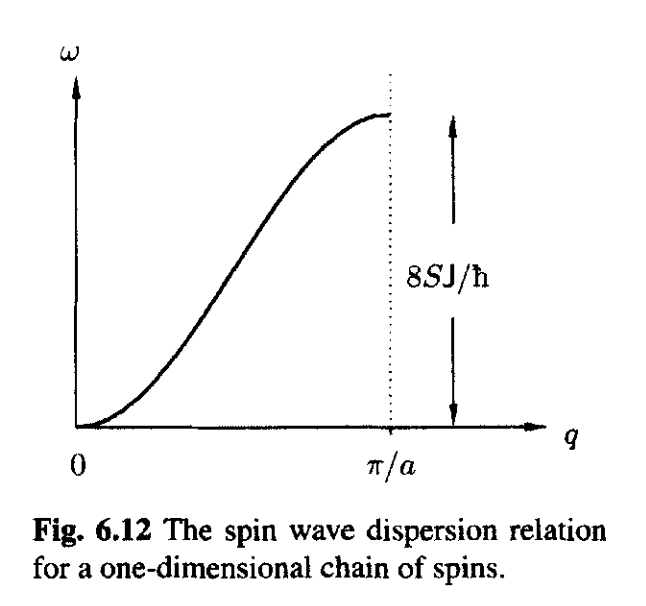
\includegraphics[height=6cm]{micm-6.12.png}
            \end{subfigure}
            \hfill
            \caption{Magnon dispersion plot from <<Magnetism in condensed matter>>.}
            \label{fig:micm-6.12}
        \end{figure}
    \end{quote}
    For the cubic system eq.~\ref{eq:micm-6.20} will look like:
    \begin{equation}
        \hbar\omega = 12JS(1 - \dfrac{1}{3}(\cos(q_xa) + \cos(q_ya) + \cos(q_za)))
    \end{equation}
    If it is to be rewritten with the notation of this paper it will look like ($n = 6$)
    \begin{equation}
        \hbar\omega = 2nJS(1 - \dfrac{1}{3}(\cos(k_xl) + \cos(k_yl) + \cos(k_zl)))
    \end{equation}

\subsection{<<Magnetisation oscillations and waves>>\cite{gurevich1996magnetization}}
    The derivation of magnon dispersion for the ferromagnet is discussed in the section~$7.4$~<<Elements of microscopic spin-wave theory>>.

    The definition of the Hamiltonian is provided on page~$205$ in equations~\eqref{eq:moaw-7.82}~and~\eqref{eq:moaw-7.82}

    \begin{quote}
        \begin{equation}
            \hatH = \gamma\hbar\sum_{f}\hat{S}_f^z - \sum_f\sum_{f^{\prime} \ne f} I_{ff^{\prime}}\mathbf{S}_f\mathbf{S}_{f^{\prime}} \label{eq:moaw-7.82} \tag{7.82}
        \end{equation}
        where $\mathbf{S}_f\mathbf{S}_{f^{\prime}} = \hat{S}_f^x\hat{S}_{f^{\prime}}^x + \hat{S}_f^y\hat{S}_{f^{\prime}}^y + \hat{S}_f^z\hat{S}_{f^{\prime}}^z$.
    \end{quote}
    The double counting is present in this Hamiltonian, thus, it is the same definition as in eq.~\eqref{eq:hh-main} of this paper with the following notation change:
    \begin{equation}
        \begin{matrix}
            f \rightarrow i, & 
            f^{\prime} \ne f \rightarrow j, & 
            I_{ff^{\prime}} \rightarrow J, & 
            \mathbf{S}_f \rightarrow \mathbf{S}_i, &
            \mathbf{S}_{f^{\prime}} \rightarrow \mathbf{S}_j
        \end{matrix}
    \end{equation}

    The dispersion law is provided in equation~\eqref{eq:moaw-7.99} on page~$209$
    \begin{quote}
        where $r_g = r_f - r_{f^{\prime}}$, $I_g \equiv I_{ff^{\prime}}$, and the last sum is over all lattice points except one, the initial. 
        The Hamiltonian ($7.98$) has the desired form of ($7.84$), and
        \begin{equation}
            \varepsilon_k(k) = \gamma\hbar H + 2S \sum_g [1 - exp(\iu \mathbf{k}\mathbf{r}_g)]I_g. \label{eq:moaw-7.99} \tag{7.99}
        \end{equation}
    \end{quote}

    For the cubic ferromagnet the textbook provides the figure~7.13 (Fig.~\ref{fig:moaw-7.13})
    \begin{quote}
        \begin{figure}[H]
            \centering
            \begin{subfigure}[b]{0.49\textwidth}
                \centering
                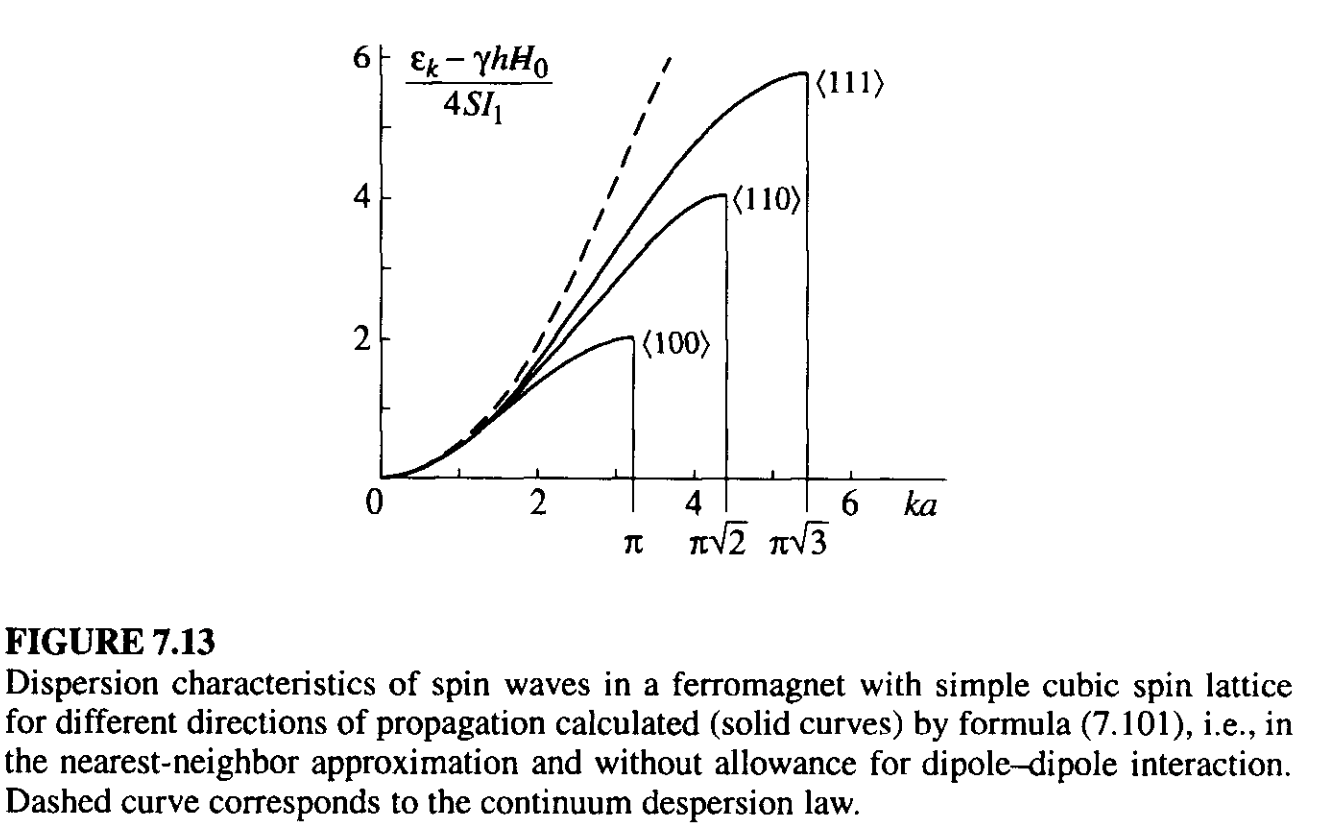
\includegraphics[height=6cm]{moaw-7.13.png}
                \caption{Original plot}
                \label{fig:moaw-7.13-original}
            \end{subfigure}
            \hfill
            \begin{subfigure}[b]{0.49\textwidth}
                \centering
                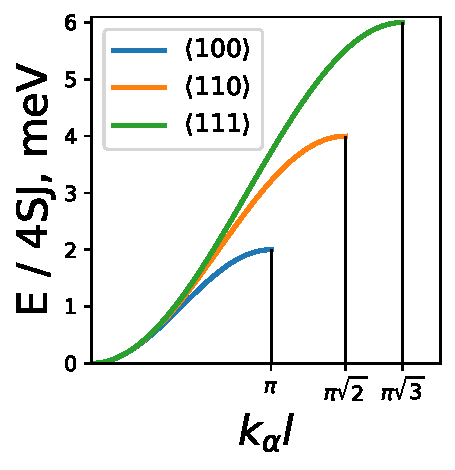
\includegraphics[height=6cm]{custom-moaw.pdf}
                \caption{Same plot with use of eq.~\eqref{eq:main-dispersion}}
                \label{fig:moaw-7.13-custom}
            \end{subfigure}
            \hfill
            \caption{Magnon dispersion plot from <<Magnetisation oscillations and waves>>.}
            \label{fig:moaw-7.13}
        \end{figure}
    \end{quote}
    In this picture curve~$\langle 100\rangle$ (from $0$ to $\pi$) corresponds to the path $\Gamma$-Y, 
    curve~$\langle 110\rangle$ (from $0$ to $\pi\sqrt{2}$) to the path $\Gamma$-M and
    curve~$\langle 111\rangle$ (from $0$ to $\pi\sqrt{3}$) to the path $\Gamma$-R 
    in the Fig.~\ref{fig:main-dispersion}. In Fig.~\ref{fig:moaw-7.13-custom} the same graph is plotted by using the equation for magnon dispersion from this paper.

    The dispersion law from eq.~\ref{eq:moaw-7.99} for the cubic system will be
    \begin{equation}
        \hbar\omega(\mathbf{k}) = 2SIn\left(1 - \dfrac{1}{3}\left(\cos(k_xr_x) + \cos(k_yr_y) + \cos(k_zr_z)\right)\right)
    \end{equation}
    where $g$ varies from $1$ to $6$ $r_g \in [r_x, -r_x, r_y, -r_y, r_z, -r_z]$ and $I_g = I$ for each $g$. 

    In the notation of this paper the dispersion law becomes ($n = 6$)
    \begin{equation}
        \hbar\omega(\mathbf{k}) = 2SJn\left(1 - \dfrac{1}{3}\left(\cos(k_xl) + \cos(k_yl) + \cos(k_zl)\right)\right)
    \end{equation}

\subsection{<<The Oxford Solid State Basics>>\cite{simon2013oxford}}
    The derivation of magnon dispersion for the ferromagnet is discussed in the exercise~$20.3$ for the Chapter~$20$~<<Spontaneous Magnetic Order: Ferro-, Antiferro-, and Ferri-Magnetism>>.

    The definition of the Hamiltonian is provided on page~$229$ in equations~\eqref{eq:ossb-20.6}~and~\eqref{eq:ossb-20.2}

    \begin{quote}
        Consider the Heisenberg Hamiltonian
        \begin{equation}
            \hatH = -\dfrac{1}{2}\sum_{\langle i,j \rangle} J \mathbf{S}_i \cdot \mathbf{S}_j + \sum_i g\mu_B \mathbf{B} \cdot \mathbf{S}_i \label{eq:ossb-20.6} \tag{20.6}
        \end{equation}
        and  for this exercise set $\mathbf{B} = 0$.
    \end{quote}

    For the first time Heisenberg Hamiltonian is defined on pages~$225-226$ in equation~\eqref{eq:ossb-20.2}
    \begin{quote}
        Note that we have included a factor of $1/2$ out front to avoid overcounting, since the sum actually counts both $J_{ij}$ and $J_{ji}$ (which are equal to each other).

        $\langle ... \rangle$

        One can use brackets $\langle i,j\rangle$ to indicate that $i$ and $j$ are neighbors:
        \begin{equation}
            \hatH = -\dfrac{1}{2}\sum_{\langle i,j \rangle} J_{ij} \mathbf{S}_i \cdot \mathbf{S}_j
        \end{equation}
        In a uniform system where each spin is coupled to its neighbors with the same strength, we can drop the indices from $J_{i,j}$ (since they all have the same value) and obtain the so-called \textit{Heisenberg Hamiltonian}
        \begin{equation}
            \hatH = -\dfrac{1}{2}\sum_{\langle i,j \rangle} J \mathbf{S}_i \cdot \mathbf{S}_j \label{eq:ossb-20.2} \tag{20.2}
        \end{equation}
        and  for this exercise set $\mathbf{B} = 0$.
    \end{quote}

    The double counting is present in this Hamiltonian, thus, it is the same definition as in eq.~\eqref{eq:hh-main} of this paper 
    with the additional factor of $1/2$, thus if we assume that definition of <<The Oxford Solid State Basics>> and this paper give the same Hamiltonian one have to 
    introduce the following substitution of exchange parameter in order to move to the definition of this paper:
    \begin{equation}
        J \rightarrow 2J \label{eq:ossb-sub}
    \end{equation}

    The dispersion law for the cubic system is provided  on page~$230$
    \begin{quote}
        $\triangleright$ Show that the dispersion curve for <<spin-waves>> of a ferromagnet is given by $\hbar\omega = \vert F(\mathbf{k})\vert$  where
        \begin{equation}
            F(\mathbf{k}) = g\mu_b\vert B \vert + JS\left(6 - 2\left(\cos(k_xa) + \cos(k_ya) + \cos(k_za)\right)\right)
        \end{equation}
        where we assume a cubic lattice
    \end{quote}

    In the notation of this paper (with the substitution~\eqref{eq:ossb-sub}) the dispersion law becomes ($n = 6$)
    \begin{equation}
        \hbar\omega(\mathbf{k}) = 2JSn\left(1 - \dfrac{1}{3}\left(\cos(k_xl) + \cos(k_yl) + \cos(k_zl)\right)\right)
    \end{equation}
\subsection{<<Magnetism and magnetic materials>>\cite{coey2010magnetism}}
    The derivation of magnon dispersion for the ferromagnet is discussed in the section~$5.4.1$~<<Spin waves>>.

    The definition of the Hamiltonian is provided on page~$137$ in equation~\eqref{eq:mamm-5.24}

    \begin{quote}
        When there is a lattice, the Hamiltonian$^1$ is generalized to a sum over all pairs of atoms on lattice sites $i, j$:
        \begin{equation}
            \hatH = -2\sum_{i > j} J_{ij} \mathbf{S}_i \cdot \mathbf{S}_j \label{eq:mamm-5.24} \tag{5.24}
        \end{equation}
    \end{quote}

    In this definition there is no double counting ($i > j$), but there is a factor of $2$ present, thus exchange constant of the Hamiltonian~\eqref{eq:mamm-5.24} are the same as in~\eqref{eq:hh-main}
    and final results for magnon dispersion are directly comparable.

    The dispersion law for the cubic system is provided  on page~$163$
    \begin{quote}
        The generalization to a three-dimensional cubic lattice with nearest-neighbour interactions is
        \begin{equation}
            \hbar \omega_q = 2JS\left[Z - \sum_{\delta}\cos\mathbf{q\cdot\delta}\right],
        \end{equation}
        where the sum is over the $Z$ vectors $\mathbf{\delta}$ connecting the central atom to its nearest neighbours.
    \end{quote}
    In case of the cubic system there is $6$ nearest-neighbours with the vectors 
    \begin{equation}
        \begin{matrix}
            (l, 0, 0),& (0, l, 0),& (0, 0, l),\\
            (-l, 0, 0),& (0, -l, 0),& (0, 0, -l),\\
        \end{matrix}
    \end{equation}
    And the dispersion law becomes:
    \begin{equation}
        \hbar \omega_q = 2JSZ\left(1 - \dfrac{1}{3}\left(\cos(q_xl) + \cos(q_yl) + \cos(q_zl)\right)\right),
    \end{equation}
    which is the same as~\eqref{eq:main-dispersion}.

\subsection{<<Rare earth magnetism>>\cite{jensen1991rare}}
    The derivation of magnon dispersion for the ferromagnet is discussed in the chapter~$5$~<<Spin waves in the ferromagnetic heavy rare earths>>.

    The definition of the Hamiltonian is provided on page~$186$ in equation~\eqref{eq:rem-5.2.1}

    \begin{quote}
        \begin{equation}
            \hatH = \sum_i\left[\sum_{l = 2,4,6}B^0_lQ_l^0(\mathbf{J}_i) + B^6_6Q_6^6(\mathbf{J}_i) - g\mu_B \mathbf{J}_i\cdot\mathbf{H}\right]
            - \dfrac{1}{2} \sum_{i\ne j} \mathcal{J}(ij)\mathbf{J} _i\cdot\mathbf{J}_j\label{eq:rem-5.2.1} \tag{5.2.1}
        \end{equation}
    \end{quote}
    
    In the equation~\eqref{eq:rem-5.2.1} crystal field and magnetic field are considered in the first sum, while the second term represents Heisenberg Hamiltonian.
    There is a double counting in the sum, thus, it is the same definition as in eq.~\eqref{eq:hh-main} of this paper 
    with the additional factor of $1/2$, therefore if we assume that definition of <<Rare earth magnetism>> and this paper give the same Hamiltonian one have to 
    introduce the following substitution of exchange parameter in order to move to the definition of this paper:
    \begin{equation}
        \mathcal{J} \rightarrow 2J \label{eq:rem-sub}
    \end{equation}

    The spin-wave spectra is defined on the page~$190$ in the equation~\eqref{eq:rem-5.2.22}
    \begin{quote}
        The energy parameters are
        \begin{equation}
            \begin{matrix}
                U_1 = \dfrac{1}{2}\sum_{\mathbf{q}}(E_{\mathbf{q}} - A_{\mathbf{q}}); & E_{\mathbf{q}} = \sqrt{A_{\mathbf{q}}^2 - B^2}.
            \end{matrix}
            \label{eq:rem-5.2.22} \tag{5.2.22}
        \end{equation}
    \end{quote}
    where $A_{\mathbf{q}}$, $A$ and $B$ are defined in the equations~\eqref{eq:rem-5.2.18} and~\eqref{eq:rem-5.2.15}
    \begin{quote}
        \begin{equation}
            \begin{matrix}
                A = \dfrac{1}{J}\left\{3B^0_2J^{(2)} - 21B^6_6J^{(6)}\cos6\phi + g\mu_BJH\cos(\phi - \phi_H)\right\}\\
                B = \dfrac{1}{J}\left\{3B^0_2J^{(2)} + 15B^6_6J^{(6)}\cos6\phi\right\}.
            \end{matrix}
            \label{eq:rem-5.2.15} \tag{5.2.15}
        \end{equation}

        $\langle ... \rangle$

        
        \begin{equation}
            A_{\mathbf{q}} = A + J\left\{\mathcal{J}(\mathbf{0}) - \mathcal{J}(\mathbf{q})\right\}
            \label{eq:rem-5.2.18} \tag{5.2.18}
        \end{equation}
    \end{quote}
    $A = 0$ and $B = 0$ if there is no magnetic field nor anisotropic effects are considered. In the case of this paper $L = 0$, thus $J = S$ and the equation for the dispersion law is
    \begin{equation}
        E_{\mathbf{q}} = S\mathcal{J}(\mathbf{0}) - \mathcal{J}(\mathbf{q})
    \end{equation}

    $\mathcal{J}(\mathbf{q})$ is defined in the equation~\eqref{eq:rem-5.1.1a}
    \begin{quote}
        \begin{equation}
            \begin{matrix}
                \mathcal{J}_{ss\prime}(\mathbf{q}) = \sum_{j \in s^{\prime} - subl.} \mathcal{J}(ij)e^{-\iu\mathbf{q}\cdot(\mathbf{R}_i - \mathbf{R}_j)}; & i \in s-sublattice,
            \end{matrix}  
            \label{eq:rem-5.1.1a} \tag{5.1.1a}
        \end{equation}
    \end{quote}
    And for the cubic lattice it becomes:
    \begin{equation}
        \mathcal{J}(\mathbf{q}) = J \left(e^{-\iu k_xl} + e^{\iu k_xl} + e^{-\iu k_yl} + e^{\iu k_yl} + e^{-\iu k_zl} + e^{\iu k_zl}\right) = 2J \left(\cos(k_xl) + \cos(k_yl) + \cos(k_zl)\right)
    \end{equation}
    And the dispersion law becomes:
    \begin{equation}
        E_{\mathbf{q}} = S(6J - 2J \left(\cos(k_xl) + \cos(k_yl) + \cos(k_zl)\right))
    \end{equation}
    In the notation of this paper after the substitution~\eqref{eq:rem-sub} formula for the dispersion law is ($n = 6$)
    \begin{equation}
        E_{\mathbf{q}} = Sn2J(1 - \dfrac{1}{3} \left(\cos(k_xl) + \cos(k_yl) + \cos(k_zl)\right))
    \end{equation}

     





    \newpage
    \bibliographystyle{plain} 
    \bibliography{refs.bib} 
    % \section*{References}
    % \printbibliography[title = {\vspace{-2em}}]



\end{document}
